\chapter{Motivácia}
AutomationShield vyvíjaný na ústave Automatizácie, merania a aplikovanej informatiky SJF STU, je open-source projekt, zameraný na vývoj hardwarových a softwarových nástrojov určených na vzdelávanie a doplnenie vzdelávacieho procesu. Jadrom celého projektu sú rozširujúce dosky(shieldy) vyvíjané pre populárny typ prototypizačných dosiek s mikrokontrolérmi Arduino, ktoré majú za ciel lepšiu výučbu strojného inžinierstva, mechatroniky a riadenia \cite{Auto}.

Ako už bolo spomenuté, hlavnou motiváciou tohoto projektu je nízka dostupnosť a vysoká cena podobných učebných pomôcok. Výučba je preto častokrát až príliš zameraná na memorovanie faktov a teórie, namiesto praktických experimentov a skúseností typu pokus-omyl. Arduino prišlo taktiež na trh v roku 2005 s úmyslom, priniesť širokej verejnosti lacnejšiu a výkonnejšiu alternatívu vtedajším mnohonásobne drahším a menej výkonným prototypizačným doskám \cite{stamp}.

Veľkou výhodou dosiek Arduino a ich nadstavbových shieldov je fakt, že sú pomerne lacné a majú malé rozmery (Arduino UNO: 68.6*53.4mm \cite{UNO} ). Tieto fakty umožňujú študentom pracovať na experimentoch nielen na pôde školy, ale experimenty si môžu zobrať domov a pracovať na nich aj mimo vyučovacieho procesu. Pre naše účely je vhodná doska Arduino UNO Obr. \ref{OBRAZOK 1.1}. Na doske sa nachádza 14 digitálnych a 6 analógových pinov. Niektoré piny sú označené špeciálnym symbolom ~, tieto piny sú schopné produkovať PWM \footnote[2]{Šírková modulácia impulzov alebo PWM je technika na dosiahnutie analógových výsledkov pomocou digitálnych prostriedkov a to, za pomoci striedania dĺžok medzi High a Low stavom resp. zapnutý a vypnutý stav.} signál ktorý potrebujeme na správne ovládanie motoru kyvadla.

\begin{figure}[!tbh]
\centering
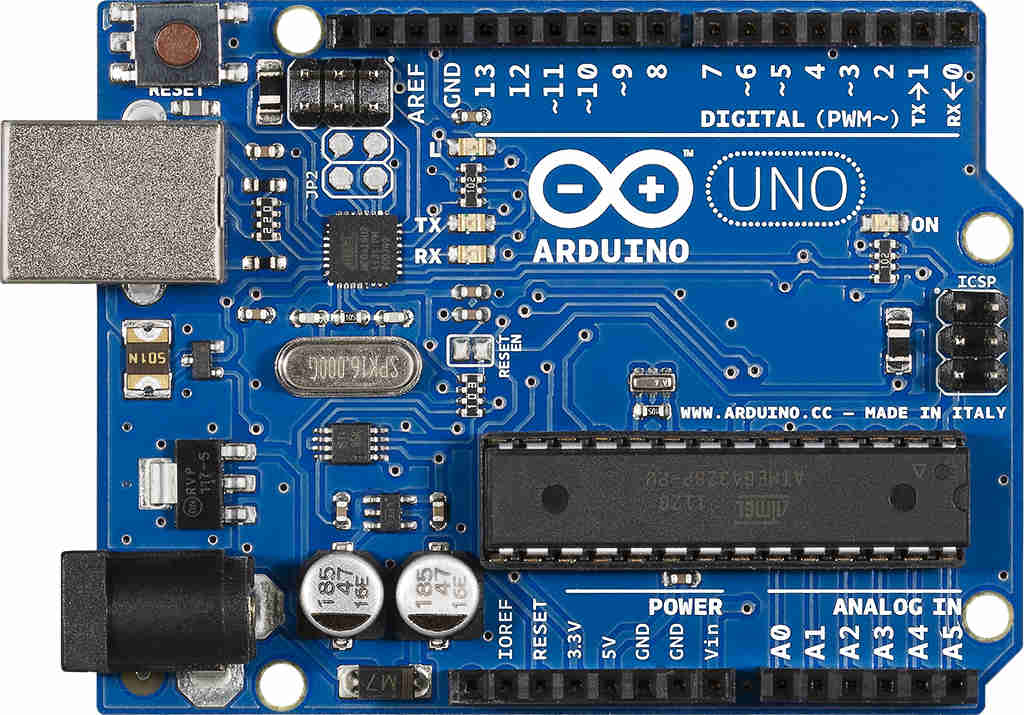
\includegraphics[width=80mm]{obr/arduino.jpg}
\caption{Arduino UNO.}\label{OBRAZOK 1.1}
\end{figure}

Cieľom tejto bakalárskej práce je návrh učebnej pomôcky, vo svete známej pod názvom Aeropendulum, čo v doslovnom preklade znamená vzdušné kyvadlo. Jedná sa o pomerne jednoduché zariadenie pozostávajúce z motorčeka, ktorý má na rotor pripojené lopatky produkujúce ťah. Motorček je zvyčajne upevnený na koniec ľahkej tyčku ktorá je v mieste otáčania pripevnená k zariadeniu na meranie uhlu pootočenia tyčky. Zariadenie na meranie pootočenia môže byť potenciometer, senzor hall efektu alebo iné \cite{senzor}. V našom prípade budeme používať senzor hall efektu ktorého fungovanie je opísané v časti hardware. Zariadenie na meranie uhlu je následne upevnené na podstavec aby sa motor mohol voľne pohybovať. Takéto kyvadlo bolo cieľom tejto bakalárskej práce a jeho podobu môžete vidieť na Obr. \ref{OBRAZOK 1.2}


\begin{figure}[!tbh]
\centering
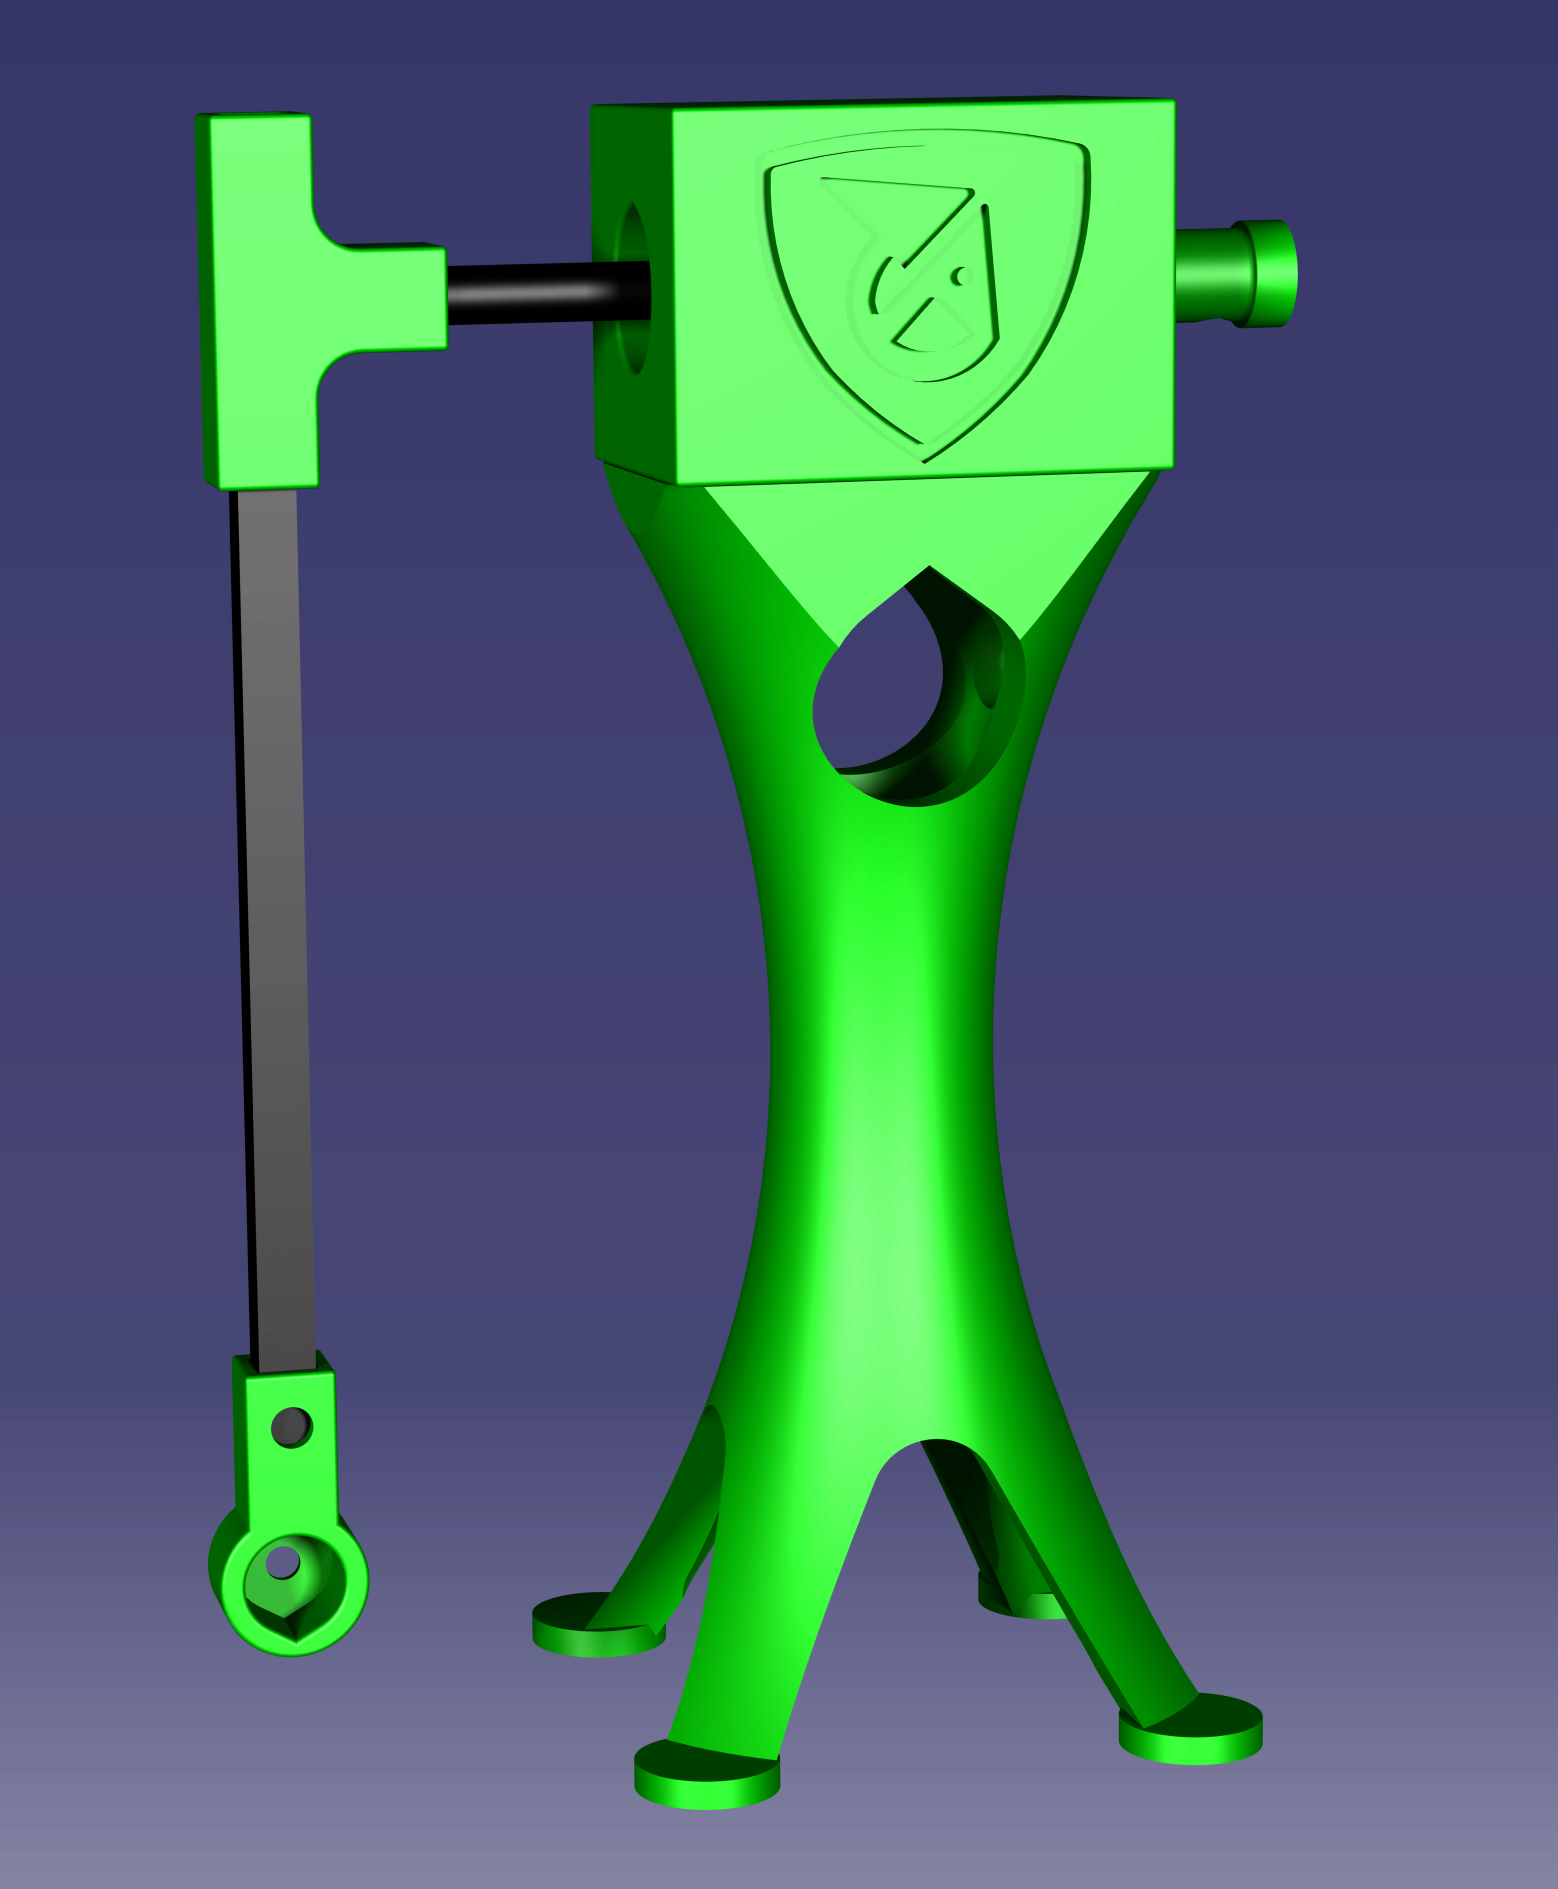
\includegraphics[width=80mm]{obr/pendulum.png}
\caption{dočasný obrázok pokial nebude hotovec final.}\label{OBRAZOK 1.2}
\end{figure}


